\documentclass[12pt]{third-rep}

\usepackage{url} % typeset URL's sensibly

\usepackage{pslatex} % Use Postscript fonts

\title{CAB402 Programming Paradigms \\ \vspace{2 mm} {Quantum Computing}}
\author{Thanat Chokwijitkul n9234900}
\date{}

\usepackage{pslatex} % sets up the use of PostScript fonts

\renewcommand{\bibname}{References} % changes to references

\usepackage{listings}

\usepackage{titlesec}
\titleformat{\chapter}{\normalfont\huge\bf}{\thechapter.}{20pt}{\huge\bf}

%% End of preamble, the actual document starts here

\begin{document}

\maketitle % creates the title

%% Generate contents etc
\tableofcontents
%\listoffigures
%\listoftables

%% These include the actual text
\chapter{Introduction}
\label{cha:intro}

\section{How to read this document}
This document attempts to do two things
\begin{itemize}
\item Provide a starting point from which you can construct your
  report.
\item Explain how one or two useful \LaTeX\ tricks work.
\end{itemize}
This means that you actually need to read it in two ways
\begin{itemize}
\item Read a printed, or previewed version to see \emph{what} can be done.
\item Read the source to see \emph{how} it's done.
\end{itemize}
If you have any comments on this document, please post them to the QandA site
 \texttt{qanda.cs.man.ac.uk}.

\section{Aim}
\label{sec:aim}

The aim of the project is to create a wonderful gismo.

A blank line is used to separate paragraphs. The chapters, sections
and subsections are numbered and added to the table of contents
automatically.

\section{Driving Latex}

\LaTeX\ is not a WYSIWYG system. You first prepare source files,
\textsf{report.tex} etc., similar to the ones here, using your
favourite text editor.

The UNIX commands you need to drive \LaTeX\ are:
\begin{enumerate}
\item \texttt{latex.} Output from \texttt{latex} can be previewed on
  the screen with \texttt{xdvi} or \texttt{gsprev} (under X), and printed on the laserprinter using  \texttt{dvips}.
  \texttt{latex} produces \textsf{.dvi} files which are used by
  \texttt{xdvi} or \texttt{gsprev} and \texttt{dvipr}.  To get all the
  cross references and the table of contents correct you sometimes
  need to run this command twice in succession.  Keep on re-running
  until the advice to rerun at the end of the output goes away.

  Many people now use \texttt{pdflatex} instead of \texttt{latex} to produce \texttt{pdf} files directly.
  
\item \texttt{xdvi} or \texttt{gsprev}. Previews the document on the
  screen, again the parameter is \textsf{report}.
  
\item \texttt{dvips.} This is used to print on the laserprinter.  The
  parameter is again \texttt{report}. 
  
\item \texttt{xfig}. Can be used to produce diagrams, see
  section~\ref{sec:diagrams}.

\end{enumerate}
There are on-line manual pages for each of the commands described above.

The set of files used to produce this document is in
\textsf{/opt/info/doc/latex} (in one of the subdirectories
\textsf{3rd-yr} or \textsf{MU-Thesis}).  They are also on the web at \url{http://csis.cs.manchester.ac.uk/software/contrib/latex/}. 

You will find that for more detailed points you will need to refer to
Lamport's `\LaTeX\ a document preparation system'~\cite{lamport}
(Copies in the library  in Blackwell's).
This example has been written using the most recent version of \LaTeX
(LaTeX2e), which is described in the \emph{2nd edition} of Lamport's
book. Buying a cheap copy of the 1st edition is probably not a good
investment. An alternative to Lamport's book, which some people
prefer, is `A guide to {\LaTeXe}' by Kopka and Daly~\cite{kopka}. The
older `A guide to {\LaTeX}'~\cite{kopka-old} by the same authors is
now obsolete. There is also pleanty of support material for \LaTeX\ on the web.

\section{Software Environment}
\subsection{Occam}

Here is some more example text, showing various \LaTeX\ facilities
you may need.  The project was mostly programmed in
\textbf{Occam}~\cite{occam}.  (A citation has been created  here to an
entry in the bibliography at the end of the report. See
chapter~\ref{cha:bib} for more details on how to do this).

Note the way of getting boldface, \textit{textit} is used for italic.
\emph{emph} is used for emphasis and is the same as italic except when
already in italic.  Note the cross reference to the bibliography.
This is how you create a footnote: DMA\footnote{Direct Memory Access.
  Footnotes can stretch over more than one line if you have a lot to
  say, but be careful not to overdo them.}.

Here is a reference to a figure. See figure~\ref{pipeline}.
\begin{figure}[htbp]
  \centering
  \setlength{\unitlength}{0.0125in}
\begin{picture}(300,35)(60,730)
\thicklines
\put(340,750){\vector( 1, 0){ 20}}
\put( 80,740){\framebox(20,20){}}
\put( 60,750){\vector( 1, 0){ 20}}
\put(100,750){\vector( 1, 0){ 20}}
\put(120,740){\framebox(20,20){}}
\put(180,750){\vector( 1, 0){ 20}}
\put(200,740){\framebox(20,20){}}
\put(160,740){\framebox(20,20){}}
\put(140,750){\vector( 1, 0){ 20}}
\put(240,740){\framebox(20,20){}}
\put(220,750){\vector( 1, 0){ 20}}
\put(260,750){\vector( 1, 0){ 20}}
\put(280,740){\framebox(20,20){}}
\put(320,740){\framebox(20,20){}}
\put(300,750){\vector( 1, 0){ 20}}
\end{picture}
  \caption{A Pipeline of processors
    \label{pipeline}}           %  this label must appear after the
                                %  \caption, and before the end of the
                                %  figure
\end{figure}
The picture in this figure was created the hard way using the picture
facility of \LaTeX. It is \emph{much} easier to use \texttt{xfig}, as
described in section~\ref{sec:diagrams}.  Whatever its contents, a
figure `floats' to a `suitable' point in the text and is never split
across a page boundary. (\LaTeX's idea of what constitutes a suitable
point may not coincide with yours)


Now we have a verbatim environment; this is a useful way of including
snippits of program, printed in a fixed width font exactly as typed:

\begin{verbatim}
{{{ An example of some folds
...  This is some folded code
  {{{ This is another fold
  This is text within the fold that has now been
  opened so that the text can be read.
  }}}
}}}
\end{verbatim}

\chapter[Short Chap title]{This chapter has a very long title that would be too long for using in headers and table of contents}
\section{Image processing}
Because Image processing is such a large topic no attempt will be made
here to describe the entire subject here but only areas directly
relevant to the project as a whole. Note how we can cross reference
sections of the document such as section~\ref{pg:filters}

\section{Low level operations}
\label{pg:filters}
Here is an example of a list with bullets:
\begin{itemize}
\item{\it Mean} Take the mean value of the neighbourhood.

\item{\it Median Filter} Take the median value of the neighbourhood.
\end{itemize}

Here are a couple of mathematical formulae:
\begin{quote}
\centering
$\Delta_1=I(x,y)-I(x+1,y+1)$ \\
$(x-a)^2+(y-b)^2=R^2$
\end{quote}

A table is just like a figure. Table~\ref{wombat} uses the tabular
environment.  Environments such as tabular can be used in ordinary
text as well.
\begin{table}
\begin{center}
\begin{tabular}{|r|c|c|c|}\hline\hline
place&1991&1992&1993\\\hline
CS Dept& 1&99&199\\
Owens Park& 1876& 22&0\\
Academy&0&0&99999\\\hline\hline
\end{tabular}
\end{center}
\caption{Distribution of Wombats in Greater Manchester}\label{wombat}
\end{table}


\section{Creating Diagrams}
\label{sec:diagrams}

Figure~\ref{fig:fig-eg} is a figure previously prepared using the
\texttt{xfig} interactive drawing package. With the latest version of
\texttt{xfig} it is quite easy to incorporate \texttt{xfig} diagrams.
The \texttt{xfig} package is menu driven and reasonably self
explanatory.

Use the \emph{Export} menu option to save an encapsulated PostScript
version of your figure, which can then be included in the document
using the \verb=\includegraphics= command. Choose the \emph{Portrait}
orientation option. For example, if the figure is in the file \textsf{
  figure1.fig}, the exporting process will create a file \textsf{
  figure1.eps}, which can then be included, scaled to whatever height
or width you want.


\begin{figure}
\begin{center}
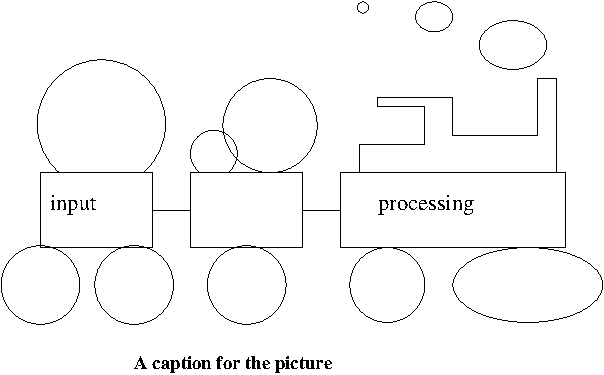
\includegraphics[width=10cm]{figure1} % This scales the picture to
                                      % a width of 10cm
                                      % You can scale to the
                                      % width or height you need
\end{center}
\caption{Final version of the system}
\label{fig:fig-eg}  
\end{figure}

Note that, if you want to use such graphics facilities in some other
document, which does not use either the \texttt{third-rep} or
\texttt{muthesis} document class, you will need to put the command
\verb=\usepackage{graphicx}= after the \verb=\documentclass....=
command in the main file.

\section{Screen Dumps}
\label{sec:screen-dumps}
\begin{figure}
\begin{center}
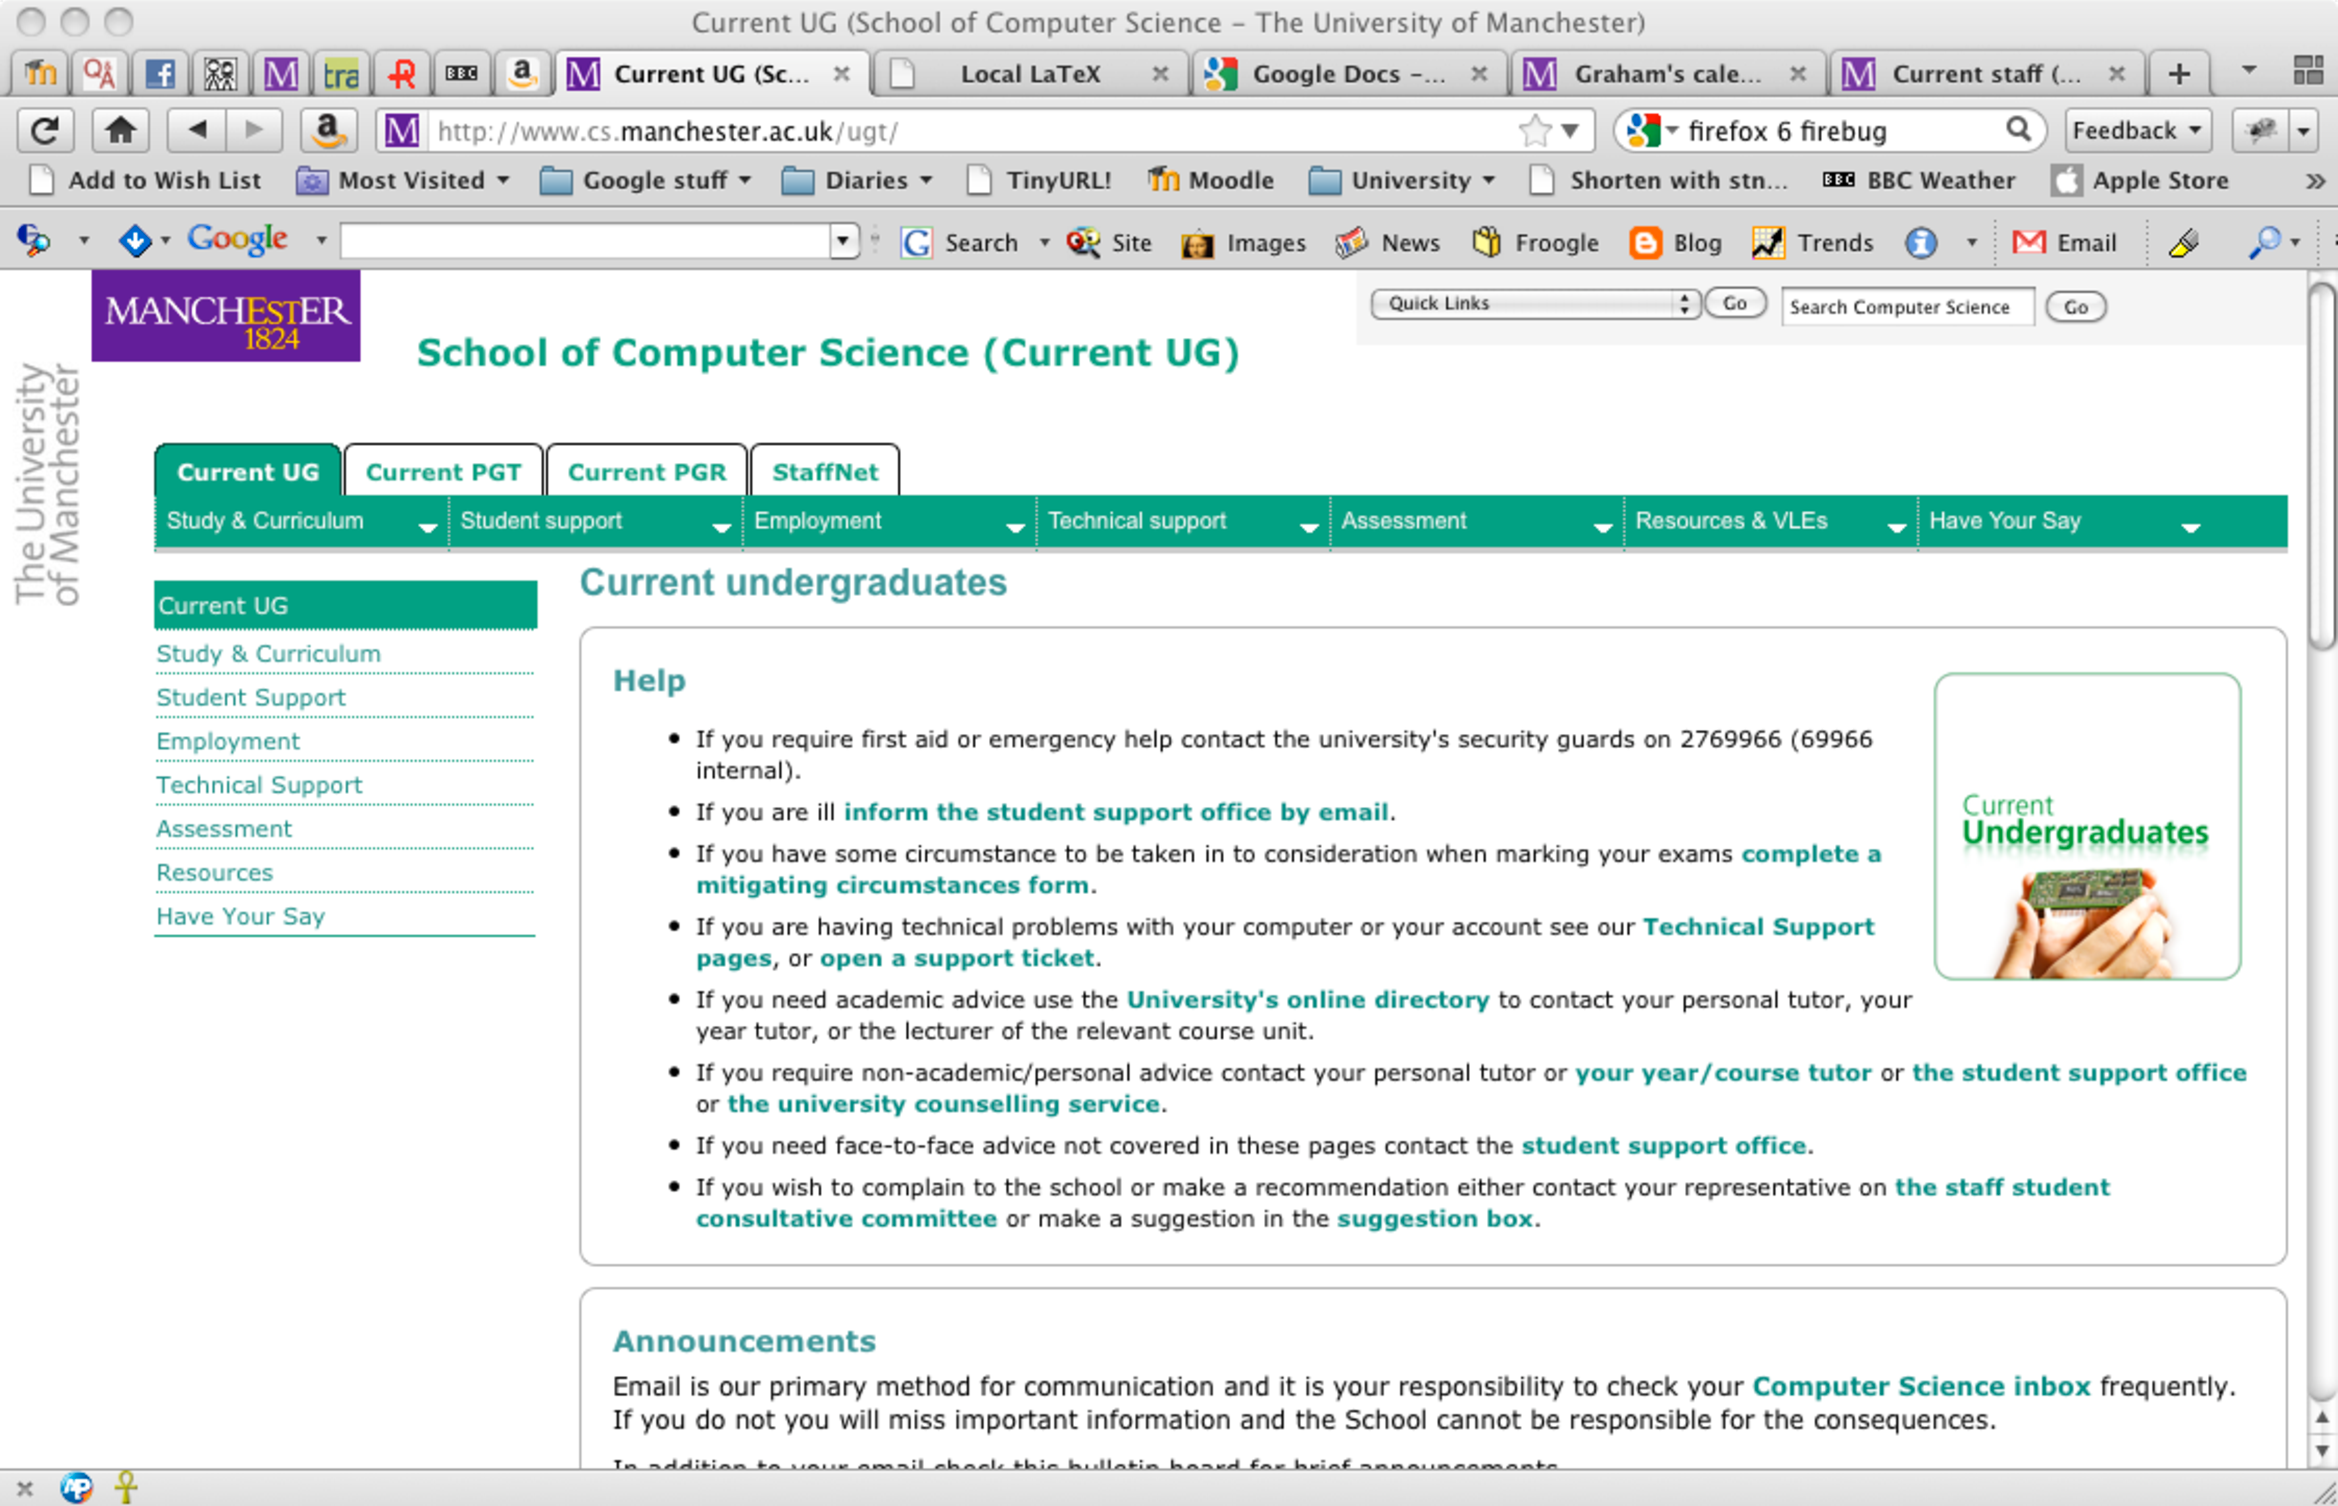
\includegraphics[width=12cm]{screen}
\end{center}
\caption{A screen dump}
\label{fig:scr-dump}
\end{figure}

Screen dumps can often enhance the appearance and clarity of a report,
although care should be taken not to overuse them. When using screen
dumps it is useful to make use of \LaTeX's capability for using
compressed PostScript files, as in the example shown in
figure~\ref{fig:scr-dump}. 

The image is first captured using, for example, \texttt{xv}, and saved
in a file, e.g.\ \texttt{screen.ps}. Next, extract the bounding box
information from the head of this file. In this case it is
\begin{verbatim}
%%BoundingBox: -100 -16 697 860
\end{verbatim}
and create a file with name given by adding \texttt{.bb} to the
original file name (in this case the name is \texttt{screen.ps.bb}) which
contains just this bounding box. You can now compress the original
file, using \texttt{gzip}. The command
\verb!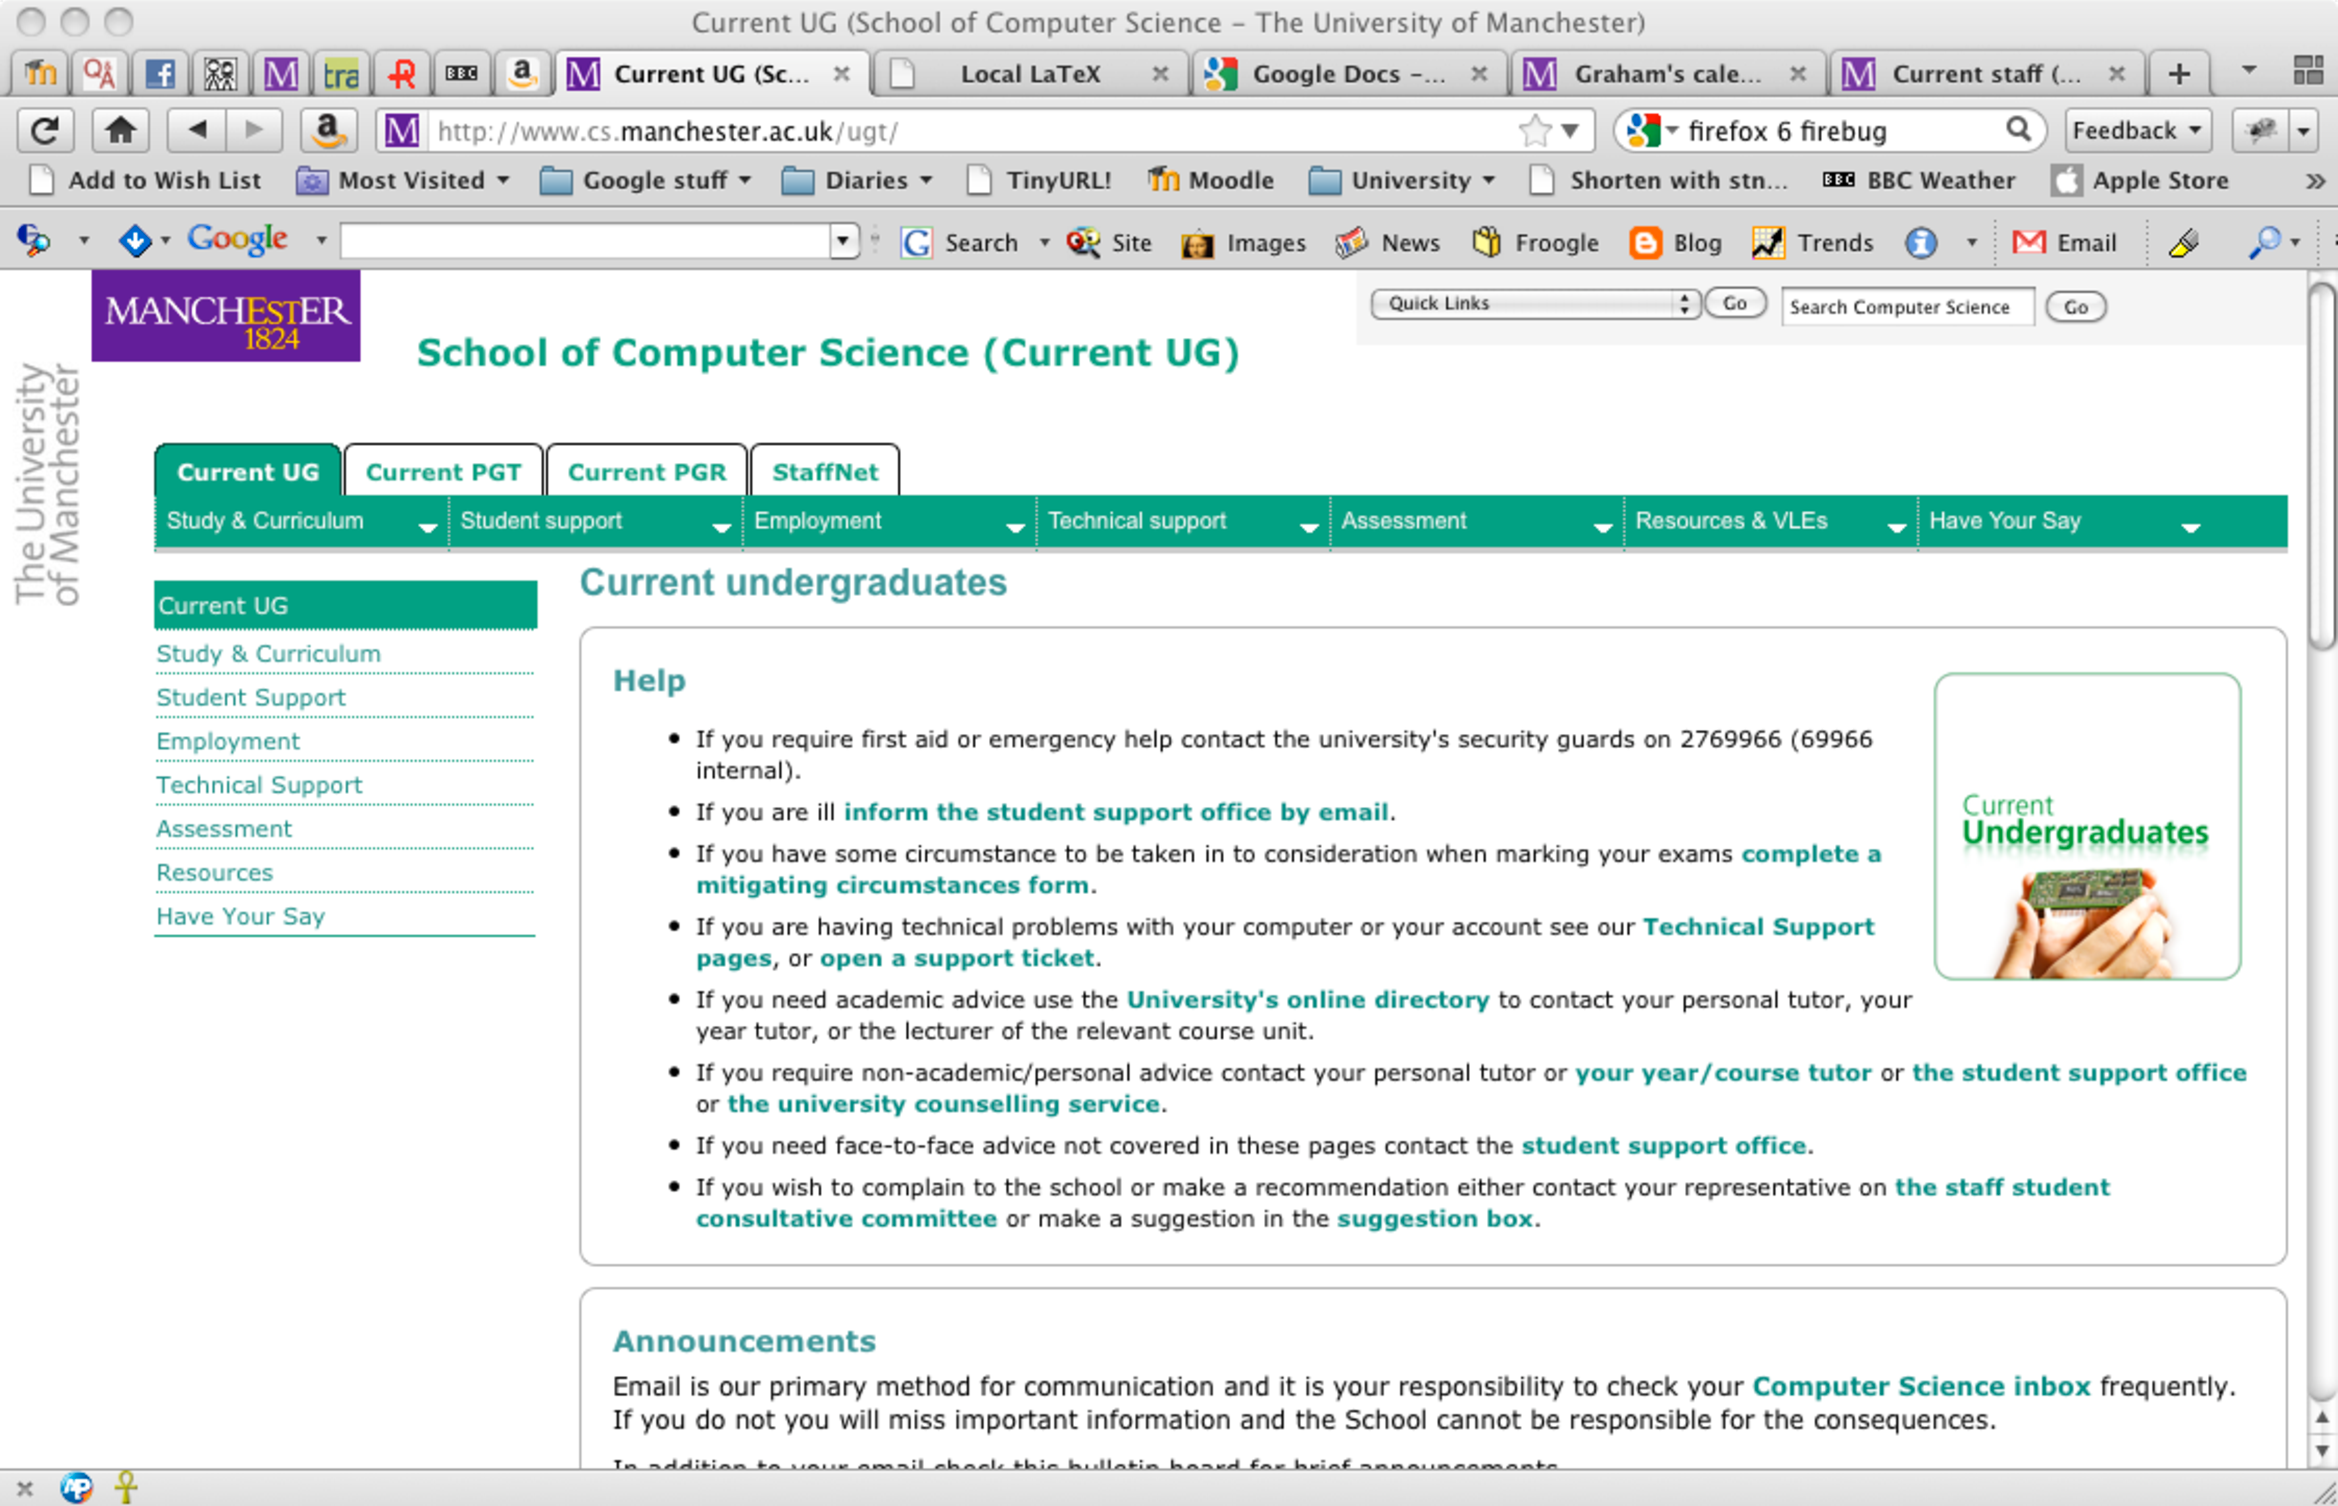
\includegraphics[width=12cm]{screen}! will look for either
\textsf{screen.ps} or \textsf{screen.ps.gz}, so you can compress or
uncompress the \textsf{ps} file without changing the latex source.

Alternatively, save as \texttt{.png} if using \texttt{pdflatex}.

The \texttt{draft} option can be used to exclude the actual figure,
but leave an appropriate amount of space.

\textbf{You may not be able to see the screen dump if you are viewing this
file from WWW. This is due to an unfortunate `feature' of the
previewer xdvi.} If you view the files directly from
\texttt{/opt/info/doc/latex/3rd-yr}, things should work properly.

\chapter{Making a bibliography}
\label{cha:bib}
Whenever you wish to refer to books or articles relevant to your report
you should use a citation such as \cite{lamport}. You can also force
entries to appear in the bibliography without  a citation appearing in
the document, by using \verb=\nocite=.  

%% This nocite produces 2 entries in the bibliography
\nocite{boyle,rd-only} 

Each document cited must have an entry in a \textsf{.bib} file. For this
document we have only one, called \textsf{refs.bib}. These files are
listed in the \verb=\bibliography= command at the end of
\textsf{report.tex}. Note that the \textsf{.bib} files can (and often
do) contain many more entries than are actually cited in a partcular
document; the only ones that appear in the bibliography are those that
have been referenced using \verb=\cite= or \verb=\nocite=.

In order to generate the appropriate reference entries, you will need
to run \texttt{bibtex} after \texttt{latex} has been run, using the
command \texttt{bibtex report}. This will generate a file
\textsf{report.bbl}, which contains the bibliography entries. Once
that file is there, you do not need to run \texttt{bibtex} again
unless you add new citations, but you will probably have to run
\texttt{latex} twice after running \texttt{bibtex} the first time.

The \TeX{} FAQ (\cite{url-cite}) gives tips on how to cite URLs.

The file \textsf{refs.bib} provides an example of what can be done
with Bib\TeX. You can find much more information in any book on
\LaTeX, for example \cite{lamport,companion,kopka}


\bibliography{refs} % this causes the references to be listed
\bibliographystyle{apalike} % bibliography style

%% Appendices start here
\appendix
\chapter{Example of operation}

An appendix is just like any other chapter, except that it comes after
the appendix command in the master file.

One use of an appendix is to include an example of input to the system
and the corresponding output.

One way to do this is to include, unformatted, an existing input file. 
You can do this using \verb=\verbatiminput=. In this appendix we
include a copy of the C file \textsf{hello.c} and its output file
\textsf{hello.out}. If you use this facility you should make sure that
the file which you input does not contain \texttt{TAB} characters,
since \LaTeX\ treats each \texttt{TAB} as a single space; you can use
the Unix command \texttt{expand} (see manual page) to expand tabs into
the appropriate number of spaces. 

\section{Example input and output}
\label{sec:inp-eg}
\subsection{Input}
\label{sec:input}
(Actually, this isn't input, it's the source code, but it will do as
an example)

\verbatiminput{hello.c}

\subsection{Output}
\label{sec:output}

\verbatiminput{hello.out}
\subsection{Another way to include code}
You can also use the capabilities of the \texttt{listings} package to
include sections of code, it does some keyword highlighting.

\lstinputlisting[language=C]{hello.c}

% Local Variables: 
% mode: latex
% TeX-master: "report"
% End:
\end{document}